\documentclass{standalone}
\usepackage[dvipsnames]{xcolor}
\usepackage{tikz}
\usetikzlibrary{calc}
\usepackage{pgfplots}
\pgfplotsset{compat=1.15}
\usepackage{mathrsfs}
\usetikzlibrary{arrows}
\usetikzlibrary[patterns]

\begin{document}
 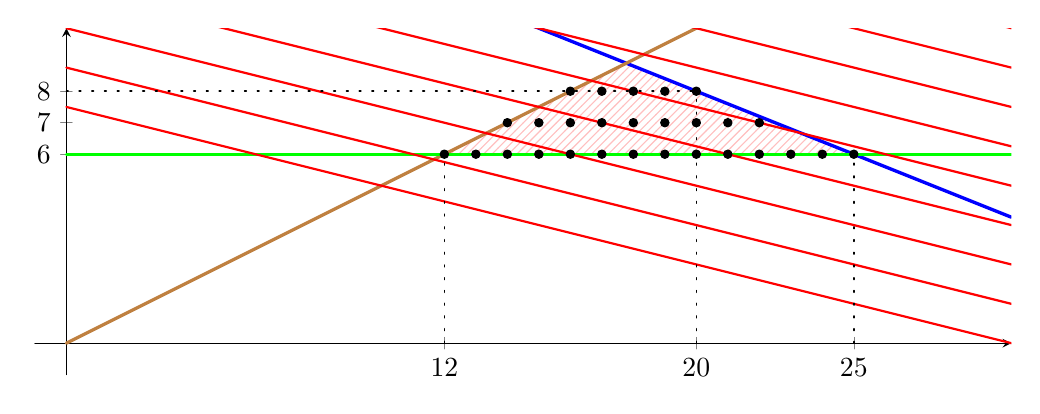
\begin{tikzpicture}[line cap=round,line join=round,>=triangle 45,x=0.4cm,y=0.4cm]
 \begin{axis}[x=0.4cm,y=0.4cm,
               axis lines=middle,
               ymajorgrids=false,
               xmajorgrids=false,
               xmin=-1,
               xmax=30,
               ymin=-1,
               ymax=10,
               xtick={12,20,25},
               ytick={6,7,8},]
 % \draw[->,color=black,line width=2.pt] (-1,0) -- (30,0);
  %\draw[->,color=black,line width=2.pt] (0,-1) -- (0,10);
  \clip(-1,-1) rectangle (30,10);
  \fill[line width=1.2pt,color=pink,fill=pink,pattern=north east lines,pattern color=pink] (12.,6.) -- (25.,6.) -- 
    (17.77777777777778,8.88888888888889) -- cycle;
  \draw [line width=1.2pt,color=blue,domain=0:30] plot(\x,{(--480.-12.*\x)/30.});
  \draw [line width=1.2pt,color=brown,domain=0:30] plot(\x,{(-0.--1.*\x)/2.});
  \draw [line width=1.2pt,color=green,domain=0:30] plot(\x,{(--6.-0.*\x)/1.});
  \draw [line width=0.8pt,color=red,domain=0:30] plot(\x,{(--3000.-100.*\x)/400.});
  \draw [line width=0.8pt,color=red,domain=0:30] plot(\x,{(--3500.-100.*\x)/400.});
  \draw [line width=0.8pt,color=red,domain=0:30] plot(\x,{(--4000.-100.*\x)/400.});
  \draw [line width=0.8pt,color=red,domain=0:30] plot(\x,{(--4500.-100.*\x)/400.});
  \draw [line width=0.8pt,color=red,domain=0:30] plot(\x,{(--5000.-100.*\x)/400.});
  \draw [line width=0.8pt,color=red,domain=0:30] plot(\x,{(--5500.-100.*\x)/400.});
  \draw [line width=0.8pt,color=red,domain=0:30] plot(\x,{(--6000.-100.*\x)/400.});
  \draw [line width=0.8pt,color=red,domain=0:30] plot(\x,{(--6500.-100.*\x)/400.});
  \draw [line width=0.8pt,color=red,domain=0:30] plot(\x,{(--7000.-100.*\x)/400.});
  \draw [fill=black] (14.,7.) circle (1.5pt);
  \draw [fill=black] (13.,6.) circle (1.5pt);
  \draw [fill=black] (12.,6.) circle (1.5pt);
  \draw [fill=black] (14.,6.) circle (1.5pt);
  \draw [fill=black] (15.,6.) circle (1.5pt);
  \draw [fill=black] (16.,6.) circle (1.5pt);
  \draw [fill=black] (17.,6.) circle (1.5pt);
  \draw [fill=black] (18.,6.) circle (1.5pt);
  \draw [fill=black] (19.,6.) circle (1.5pt);
  \draw [fill=black] (20.,6.) circle (1.5pt);
  \draw [fill=black] (21.,6.) circle (1.5pt);
  \draw [fill=black] (22.,6.) circle (1.5pt);
  \draw [fill=black] (23.,6.) circle (1.5pt);
  \draw [fill=black] (24.,6.) circle (1.5pt);
  \draw [fill=black] (25.,6.) circle (1.5pt);
  \draw [fill=black] (22.,7.) circle (1.5pt);
  \draw [fill=black] (21.,7.) circle (1.5pt);
  \draw [fill=black] (20.,7.) circle (1.5pt);
  \draw [fill=black] (19.,7.) circle (1.5pt);
  \draw [fill=black] (18.,7.) circle (1.5pt);
  \draw [fill=black] (17.,7.) circle (1.5pt);
  \draw [fill=black] (16.,7.) circle (1.5pt);
  \draw [fill=black] (15.,7.) circle (1.5pt);
  \draw [fill=black] (16.,8.) circle (1.5pt);
  \draw [fill=black] (17.,8.) circle (1.5pt);
  \draw [fill=black] (18.,8.) circle (1.5pt);
  \draw [fill=black] (19.,8.) circle (1.5pt);
  \draw [fill=black] (20.,8.) circle (1.5pt);
\draw[color=black,line width=0.6pt,loosely dotted] (12,0) -- (12,6);
\draw[color=black,line width=0.6pt,loosely dotted] (20,0) -- (20,8);
\draw[color=black,line width=0.6pt,loosely dotted] (25,0) -- (25,6);
\draw[color=black,line width=0.6pt,loosely dotted] (0,8) -- (20,8);
  \end{axis}
 \end{tikzpicture}
\end{document}

